\documentclass[UKenglish]{beamer}


\usetheme{UiB}

\usepackage{algorithm}
\usepackage[noend]{algpseudocode}
\usepackage[utf8]{inputenx} % For æ, ø, å
\usepackage{csquotes}       % Quotation marks
\usepackage{microtype}      % Improved typography
\usepackage{amssymb}        % Mathematical symbols
\usepackage{mathtools}      % Mathematical symbols
\usepackage[absolute, overlay]{textpos} % Arbitrary placement
\setlength{\TPHorizModule}{\paperwidth} % Textpos units
\setlength{\TPVertModule}{\paperheight} % Textpos units
\usepackage{tikz}
\usetikzlibrary{overlay-beamer-styles}  % Overlay effects for TikZ


\author{Kate\v{r}ina \v{C}\'{i}\v{z}kov\'{a}, Luca Klingenberg}
\title{Parallel Matrix Multiplication}
\subtitle{Final Project\\ INF236: Parallel Programming}


\begin{document}


\section{Introduction}
% Use
%
%     \begin{frame}[allowframebreaks]{Title}
%
% if the TOC does not fit one frame.
\begin{frame}{Table of contents}
    \tableofcontents[currentsection]
\end{frame}

\begin{frame}{Introduction}
	\begin{itemize}
        \item
        Complexity: $\mathcal{O}(n^3)$
        \item 
        Consecutive memory access
    \end{itemize}
    
	\begin{algorithm}[H] 
\caption{matrix multiplication}
\label{alg:matmul}
\begin{algorithmic}[1]
\Require{$\mathbf{A}, \mathbf{B}$} %Input
\Ensure{$\mathbf{C}$ (the resulting matrix)} %Output
\Statex
\Function{matmul}{$\mathbf{A}, \mathbf{B}$}
	\For{$i=0, \ldots, n-1$}
		\For {$j=0, \ldots, n-1$}
			\State {$c[i][j] = 0$}
		\EndFor
		\For{$k=0, \ldots, n-1$}
			\For{$j=0, \ldots, n-1$}
				\State {$c[i][j] += a[i][k] \cdot b[k][j]$}
			\EndFor
		\EndFor
	\EndFor
	\State \Return {$\mathbf{C}$}
\EndFunction
\end{algorithmic}
\end{algorithm}
\end{frame}

\section{Strassen's Algorithm}

\begin{frame}{Strassen's Algorithm}

\begin{itemize}
        \item
        Blockwise matrix multiplication
        \begin{align*}
\mathbf{A} \cdot \mathbf{B} &=
\begin{pmatrix}
\mathbf{A}_{00} & \mathbf{A}_{01} \\
\mathbf{A}_{10} & \mathbf{A}_{11} 
\end{pmatrix}
\cdot
\begin{pmatrix}
\mathbf{B}_{00} & \mathbf{B}_{01} \\
\mathbf{B}_{10} & \mathbf{B}_{11} 
\end{pmatrix} \\
&=
\begin{pmatrix}
\mathbf{A}_{00}\mathbf{B}_{00}+\mathbf{A}_{01}\mathbf{B}_{10} & \mathbf{A}_{00}\mathbf{B}_{01}+\mathbf{A}_{01}\mathbf{B}_{11} \\
\mathbf{A}_{10}\mathbf{B}_{00}+\mathbf{A}_{11}\mathbf{B}_{10} & \mathbf{A}_{10}\mathbf{B}_{01}+\mathbf{A}_{11}\mathbf{B}_{11} 
\end{pmatrix} \\
&=
\begin{pmatrix}
\mathbf{C}_{00} & \mathbf{C}_{01} \\
\mathbf{C}_{10} & \mathbf{C}_{11} 
\end{pmatrix}
= \mathbf{C}
\end{align*}
	\item 
     Idea: reduce number of multiplications from 8 to 7
     \item 
     Complexity of Strassen's algorithm: 
    $\mathcal{O}(n^{\log_2{7}}) \approx \mathcal{O}(n^{2.8073})$
    \end{itemize}
\end{frame}


\begin{frame}{Strassen's Algorithm}
\begin{center}
    \scalebox{0.75}{
    \begin{minipage}{0.7\linewidth}
\begin{algorithm}[H] 
\caption{Strassen's matrix multiplication}
\label{alg:strassen}
\begin{algorithmic}[1]
\Require{$\mathbf{A}, \mathbf{B}$} %Input
\Ensure{$\mathbf{C}$ (the resulting matrix)} %Output
\Statex
\Function{strassen}{$\mathbf{A}, \mathbf{B}, n$}
	\If {n == cutoff}
		\State \Return \Call{matmul}{$\mathbf{A}, \mathbf{B}$}
	\EndIf
	\State {$\mathbf{P}_1 = \Call{strassen}{\mathbf{A}_{00} + \mathbf{A}_{11},  \mathbf{B}_{00} + \mathbf{B}_{11}, \frac{n}{2}$}}
	\State {$\mathbf{P}_2 = \Call{strassen}{\mathbf{A}_{10} + \mathbf{A}_{11},  \mathbf{B}_{00}, \frac{n}{2}$}}
	\State {$\mathbf{P}_3 = \Call{strassen}{\mathbf{A}_{00},  \mathbf{B}_{01} - \mathbf{B}_{11}, \frac{n}{2}$}}
	\State {$\mathbf{P}_4 = \Call{strassen}{\mathbf{A}_{11},  \mathbf{B}_{10} - \mathbf{B}_{00}, \frac{n}{2}$}}
	\State {$\mathbf{P}_5 = \Call{strassen}{\mathbf{A}_{00} + \mathbf{A}_{01},  \mathbf{B}_{11}, \frac{n}{2}$}}
	\State {$\mathbf{P}_6 = \Call{strassen}{\mathbf{A}_{10} - \mathbf{A}_{00},  \mathbf{B}_{00} + \mathbf{B}_{01}, \frac{n}{2}$}}
	\State {$\mathbf{P}_7 = \Call{strassen}{\mathbf{A}_{01} - \mathbf{A}_{11},  \mathbf{B}_{10} + \mathbf{B}_{11}, \frac{n}{2}$}}
	\State {$\mathbf{C}_{00} = \mathbf{P}_1 + \mathbf{P}_4 - \mathbf{P}_5 + \mathbf{P}_7$}
	\State {$\mathbf{C}_{01} = \mathbf{P}_3 + \mathbf{P}_5$}
	\State {$\mathbf{C}_{10} = \mathbf{P}_2 + \mathbf{P}_4$}
	\State {$\mathbf{C}_{11} = \mathbf{P}_1 - \mathbf{P}_2 + \mathbf{P}_3 + \mathbf{P}_6$}
	\State \Return {$\mathbf{C}$}
\EndFunction
\end{algorithmic}
\end{algorithm}
\end{minipage}%
    }
  \end{center}
\end{frame}

\subsection{z-ordering}

\begin{frame}{z-ordering}
	\vspace{0.5cm}
	\begin{figure}[htbp]
\centerline{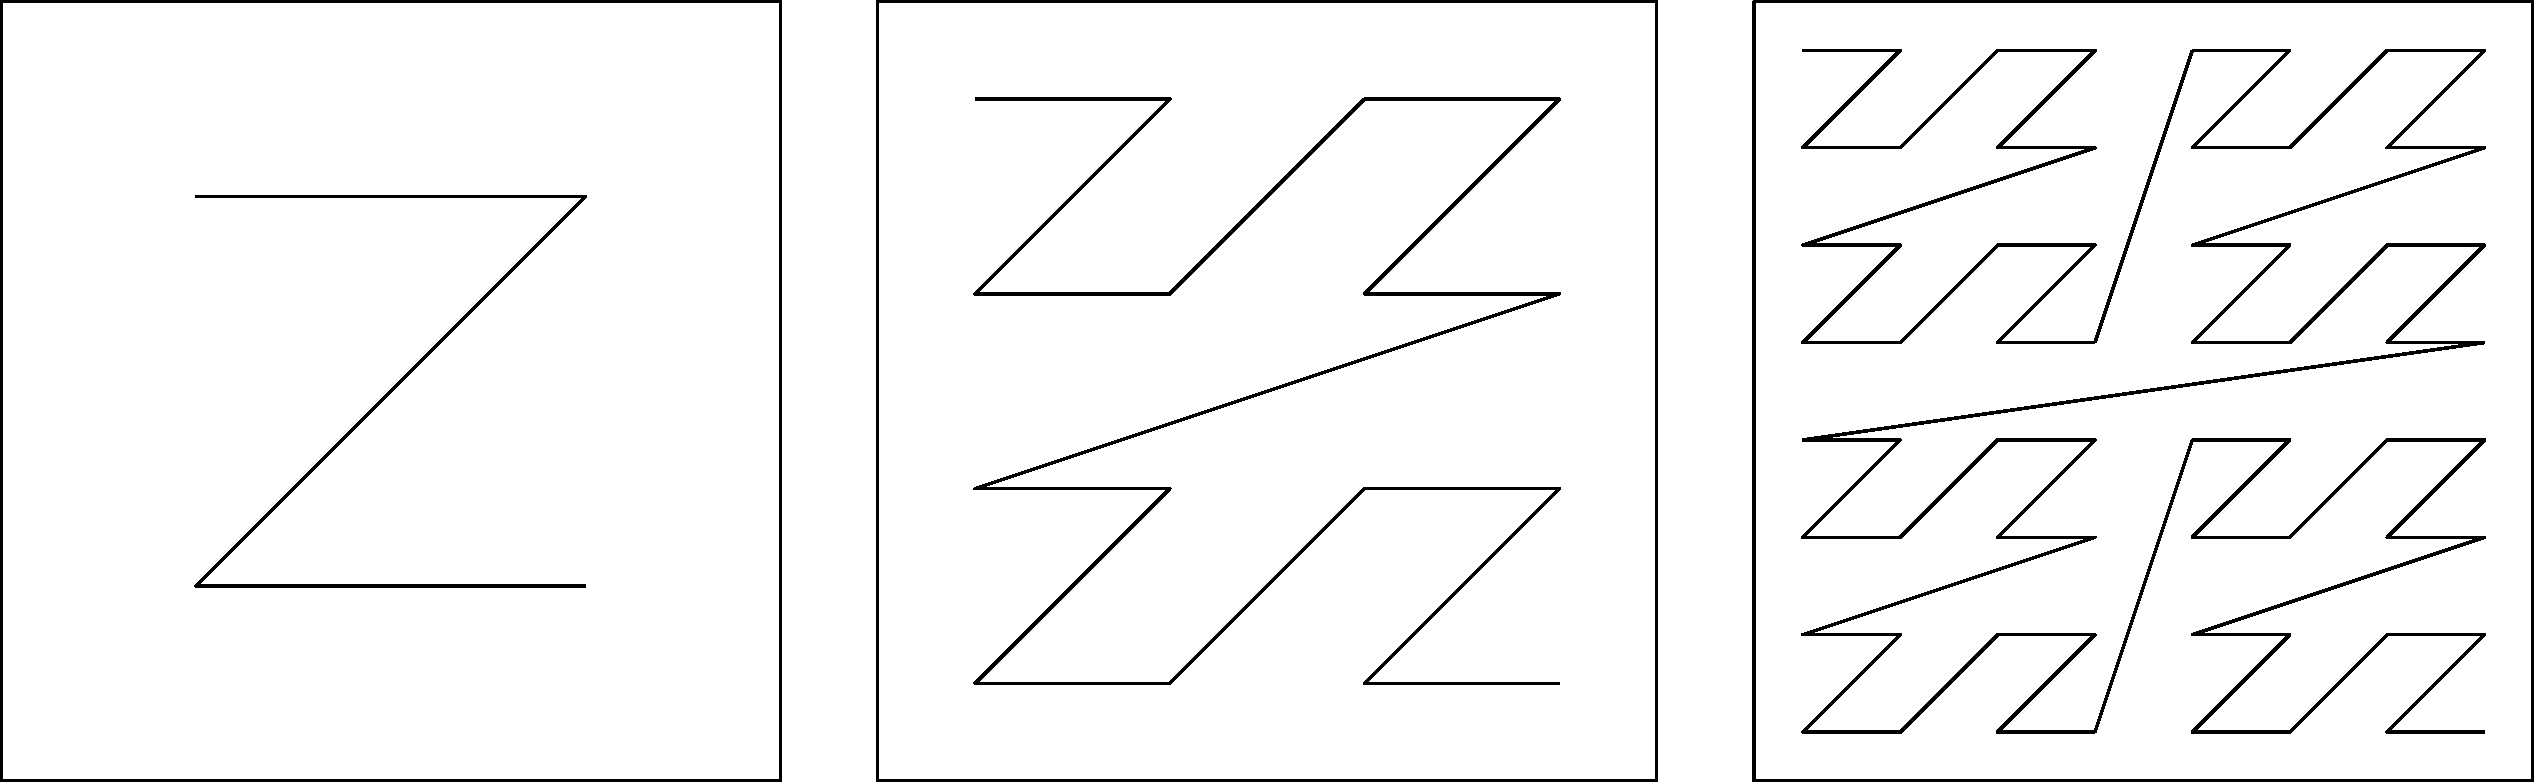
\includegraphics[scale=.16]{z_ordering.pdf}}
\centerline{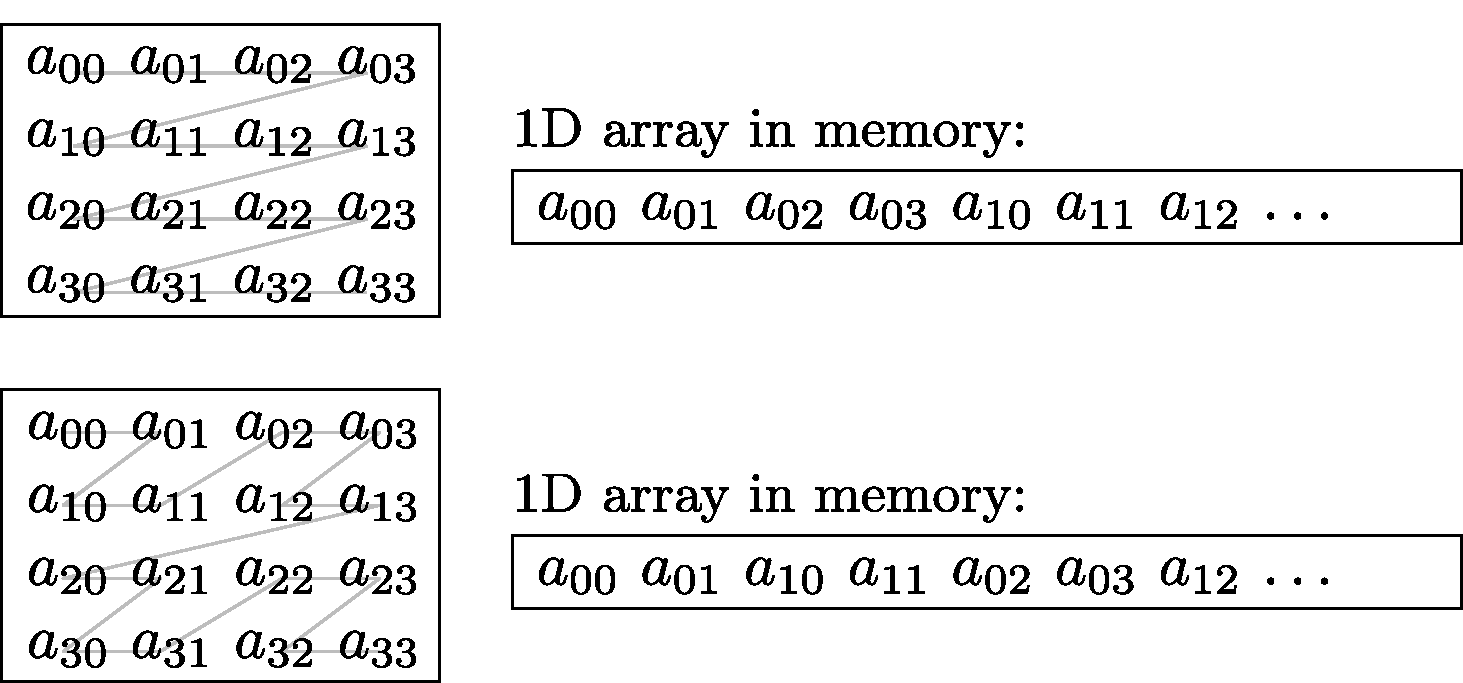
\includegraphics[scale=.2775]{mem_ordering.pdf}}
\end{figure}
\end{frame}

\begin{frame}{z-ordering}
\begin{itemize}
		\item
		Matrices at cutoff level are stored row-wise
		\vspace{0.25cm}
			\begin{figure}[htbp]
				\centerline{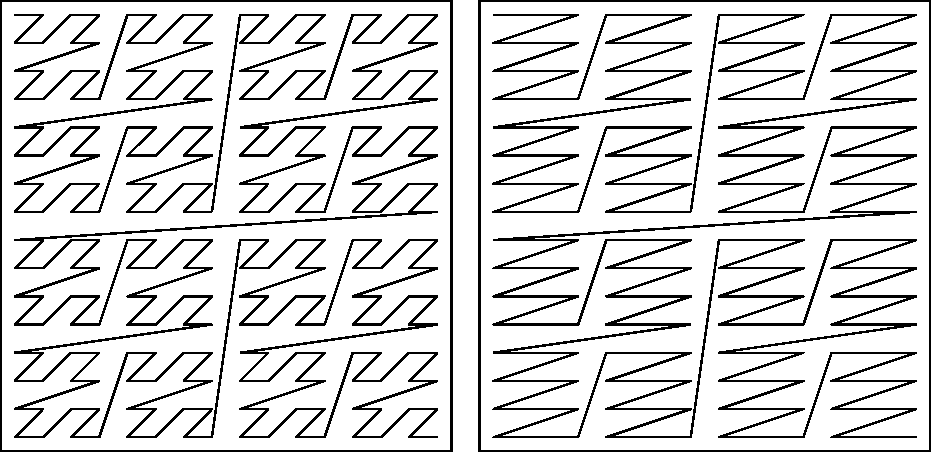
\includegraphics[scale=.5]{partly_z_ordering.pdf}}
			\end{figure}
		\item
		
		\end{itemize}
\end{frame}


\section{Experiments}

\begin{frame}{Experiments}

\end{frame}

\section{Conclusion}

\begin{frame}{Conclusion}

\end{frame}


\if{}
\section{Mathematics}
\subsection{Theorem}


\begin{frame}{Mathematics}
    \begin{theorem}[Fermat's little theorem]
        For a prime~\(p\) and \(a \in \mathbb{Z}\) it holds that \(a^p \equiv a \pmod{p}\).
    \end{theorem}

    \begin{proof}
        The invertible elements in a field form a group under multiplication.
        In particular, the elements
        \begin{equation*}
            1, 2, \ldots, p - 1 \in \mathbb{Z}_p
        \end{equation*}
        form a group under multiplication modulo~\(p\).
        This is a group of order \(p - 1\).
        For \(a \in \mathbb{Z}_p\) and \(a \neq 0\) we thus get \(a^{p-1} = 1 \in \mathbb{Z}_p\).
        The claim follows.
    \end{proof}
\end{frame}


\subsection{Example}


\begin{frame}{Mathematics}
    \begin{example}
        The function \(\phi \colon \mathbb{R} \to \mathbb{R}\) given by \(\phi(x) = 2x\) is continuous at the point \(x = \alpha\),
        because if \(\epsilon > 0\) and \(x \in \mathbb{R}\) is such that \(\lvert x - \alpha \rvert < \delta = \frac{\epsilon}{2}\),
        then
        \begin{equation*}
            \lvert \phi(x) - \phi(\alpha)\rvert = 2\lvert x - \alpha \rvert < 2\delta = \epsilon.
        \end{equation*}
    \end{example}
\end{frame}


\section{Highlighting}
\SectionPage


\begin{frame}{Highlighting}
    Sometimes it is useful to \alert{highlight} certain words in the text.

    \begin{alertblock}{Important message}
        If a lot of text should be \alert{highlighted}, it is a good idea to put it in a box.
    \end{alertblock}

    It is easy to match the \structure{colour theme}.
\end{frame}


\section{Lists}


\begin{frame}{Lists}
    \begin{itemize}
        \item
        Bullet lists are marked with a red box.
    \end{itemize}

    \begin{enumerate}
        \item
        \label{enum:item}
        Numbered lists are marked with a white number inside a red box.
    \end{enumerate}

    \begin{description}
        \item[Description] highlights important words with red text.
    \end{description}

    Items in numbered lists like \enumref{enum:item} can be referenced with a red box.

    \begin{example}
        \begin{itemize}
            \item
            Lists change colour after the environment.
        \end{itemize}
    \end{example}
\end{frame}


\section{Effects}


\begin{frame}{Effects}
    \begin{columns}[onlytextwidth]
        \begin{column}{0.49\textwidth}
            \begin{enumerate}[<+-|alert@+>]
                \item
                Effects that control

                \item
                when text is displayed

                \item
                are specified with <> and a list of slides.
            \end{enumerate}

            \begin{theorem}<2>
                This theorem is only visible on slide number 2.
            \end{theorem}
        \end{column}
        \begin{column}{0.49\textwidth}
            Use \textbf<2->{textblock} for arbitrary placement of objects.

            \pause
            \medskip

            It creates a box
            with the specified width (here in a percentage of the slide's width)
            and upper left corner at the specified coordinate (x, y)
            (here x is a percentage of width and y a percentage of height).
        \end{column}
    \end{columns}
    
    \begin{textblock}{0.3}(0.45, 0.55)
        \includegraphics<1, 3>[width = \textwidth]{UiB-images/UiB-emblem}
    \end{textblock}
\end{frame}


\section{References}


\begin{frame}[allowframebreaks]{References}
    \begin{thebibliography}{}

        % Article is the default.
        \setbeamertemplate{bibliography item}[book]

        \bibitem{Hartshorne1977}
        Hartshorne, R.
        \newblock \emph{Algebraic Geometry}.
        \newblock Springer-Verlag, 1977.

        \setbeamertemplate{bibliography item}[article]

        \bibitem{Helso2020}
        Helsø, M.
        \newblock \enquote{Rational quartic symmetroids}.
        \newblock \emph{Adv. Geom.}, 20(1):71--89, 2020.

        \setbeamertemplate{bibliography item}[online]

        \bibitem{HR2018}
        Helsø, M.\ and Ranestad, K.
        \newblock \emph{Rational quartic spectrahedra}, 2018.
        \newblock \url{https://arxiv.org/abs/1810.11235}

        \setbeamertemplate{bibliography item}[triangle]

        \bibitem{AM1969}
        Atiyah, M.\ and Macdonald, I.
        \newblock \emph{Introduction to commutative algebra}.
        \newblock Addison-Wesley Publishing Co., Reading, Mass.-London-Don
        Mills, Ont., 1969

        \setbeamertemplate{bibliography item}[text]

        \bibitem{Artin1966}
        Artin, M.
        \newblock \enquote{On isolated rational singularities of surfaces}.
        \newblock \emph{Amer. J. Math.}, 80(1):129--136, 1966.

    \end{thebibliography}
\end{frame}

\fi{}

\end{document}